
\section{Results}
\label{sec_results}

% FIXME: If you can, put a paragraph summarizing this section here so that
% the section heading is not immediately followed by the subsection heading.
% Fan wrote the following.

We formalise the metrics we use to compare multi-objective optimisation approaches in this section.
The results are presented in Section~\ref{sec_answers}, and are used to answer the \textbf{RQ}s.

\subsection{Metrics}
\label{sec_matrics}

To investigate RQ1 and RQ2, we collect the non-dominated set of solutions from each algorithm for 20 runs, and report it in an attainment surface as introduced by Fonseca~\cite{attainment_surface:1996}. To quantitatively compare the quality of each algorithm, we calculate Hypervolume and Contribution indicators to assess the multi-objective Pareto Front.

\textbf{Hypervolume}: The Hypervolume indicator~\cite{797969} measures the space dominated by the solutions. It is defined as the hypervolume of the union of hypercubes dominated by each solution on the Front. The bigger the Hypervolume is, the larger the area dominated by the Pareto Front in the objective space is, and thus the better the performance is.

\textbf{Contribution}: Since there is no way to know the true Pareto Front, we use the non-dominated set of joint solutions from all experiments to approximate the true Pareto Front, forming a `reference' front. The Contribution indicator represents the ratio of solutions on the reference front that are found by a given algorithm. A higher ratio indicates a more successful search. 

To allow comparison across subject programs, objectives are normalised to the original performance of each subject.

\subsection{Answers to RQs}
\label{sec_answers}

\newcommand{\shallow}{Sha}
\newcommand{\all}{All}
\newcommand{\randomsearch}{Rand}
\newcommand{\nsgaii}{NSGA}
\newcommand{\sr}{\emph{\shallow\randomsearch}}
\newcommand{\sn}{\emph{\shallow\nsgaii}}
\newcommand{\dr}{\emph{\all\randomsearch}}
\newcommand{\dn}{\emph{\all\nsgaii}}

For brevity we use \emph{\shallow} to refer to shallow parameters and \emph{\all} to refer to all parameters including shallow and deep parameters, followed by \emph{\randomsearch} or \emph{\nsgaii} to indicate the search method used (random search or NSGA-II). For example, \sn{} refers to using NSGA-II to search for better values for shallow parameters.
%In subsequent graphs, the performance of the original program always locates at (1, 1) since all the performance is normalised to it.

\begin{figure*}[htb]
	\centering
	\subfigure[espresso]{
		\label{fig_attainment_espresso}
		\scalebox{1}{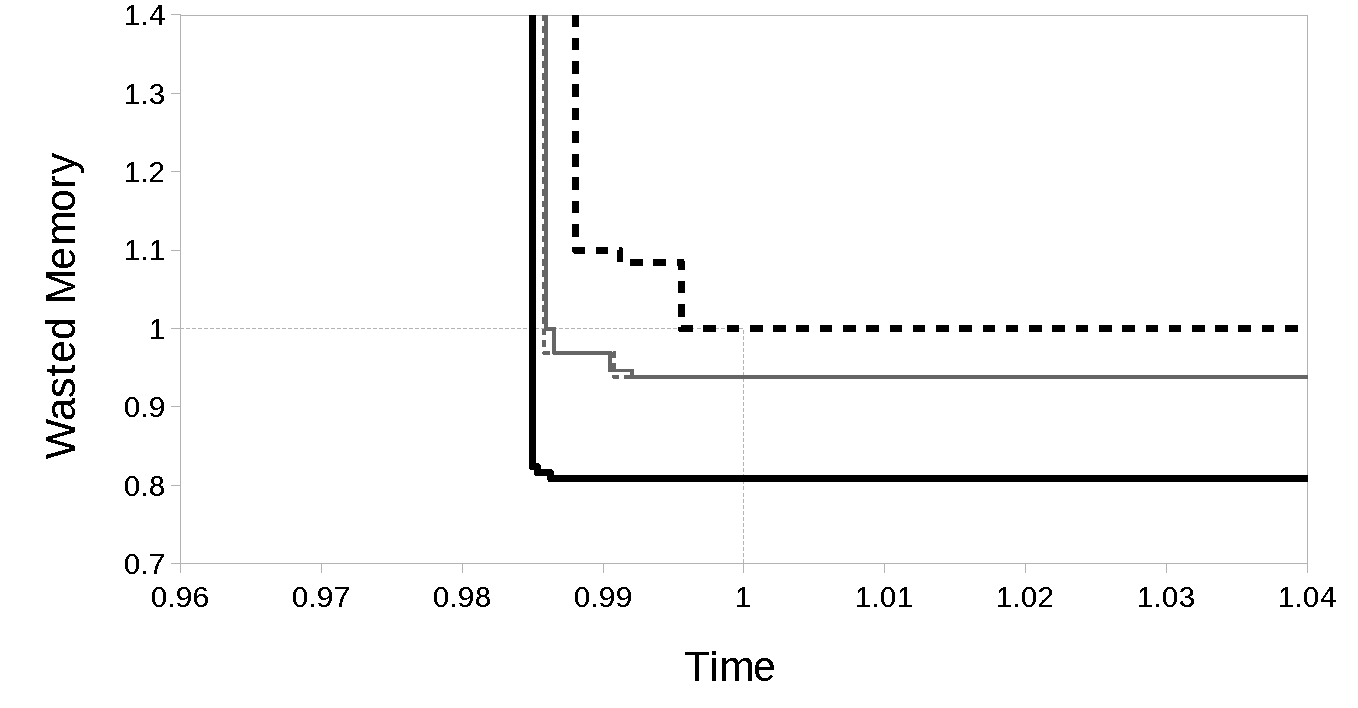
\includegraphics[width=0.47\textwidth]{espresso_attainment_pdf}}
	}
	\subfigure[gawk]{
		\label{fig_attainment_gawk}
		\scalebox{1}{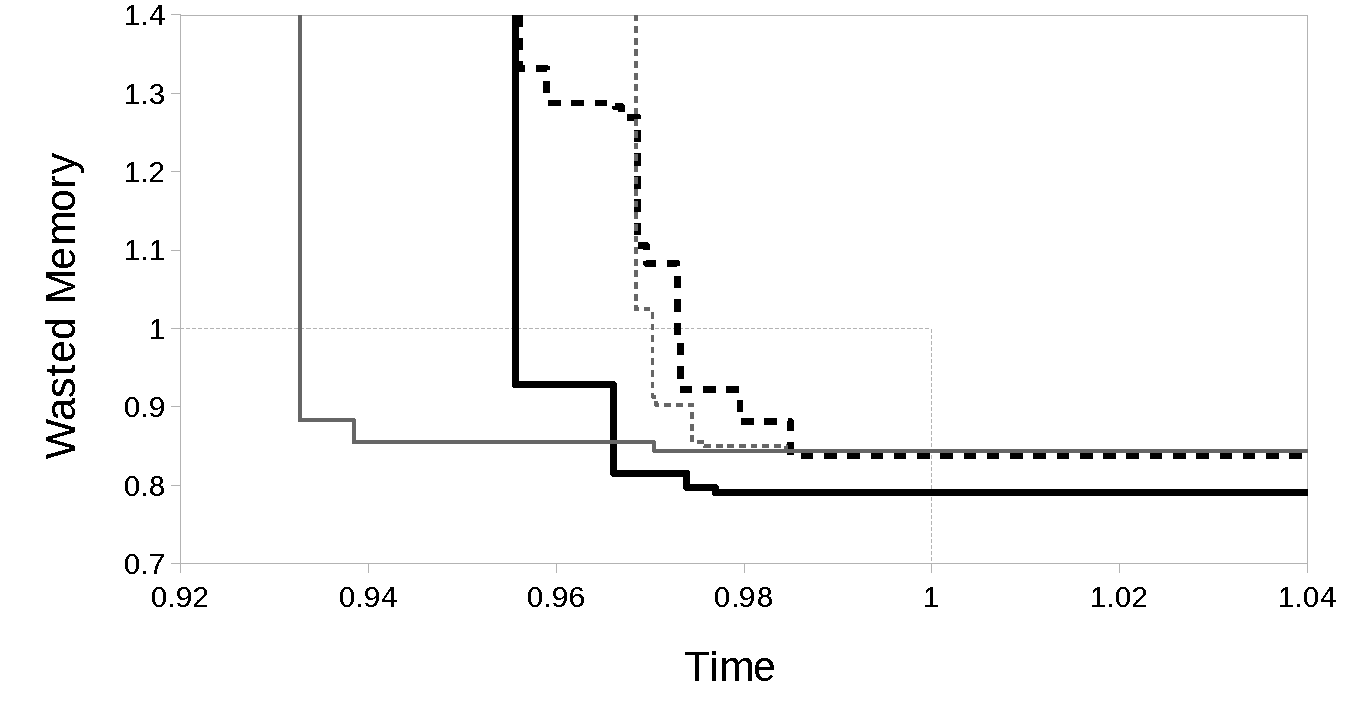
\includegraphics[width=0.47\textwidth]{gawk_attainment_pdf}}
	}
	\subfigure[flex]{
		\label{fig_attainment_flex}
		\scalebox{1}{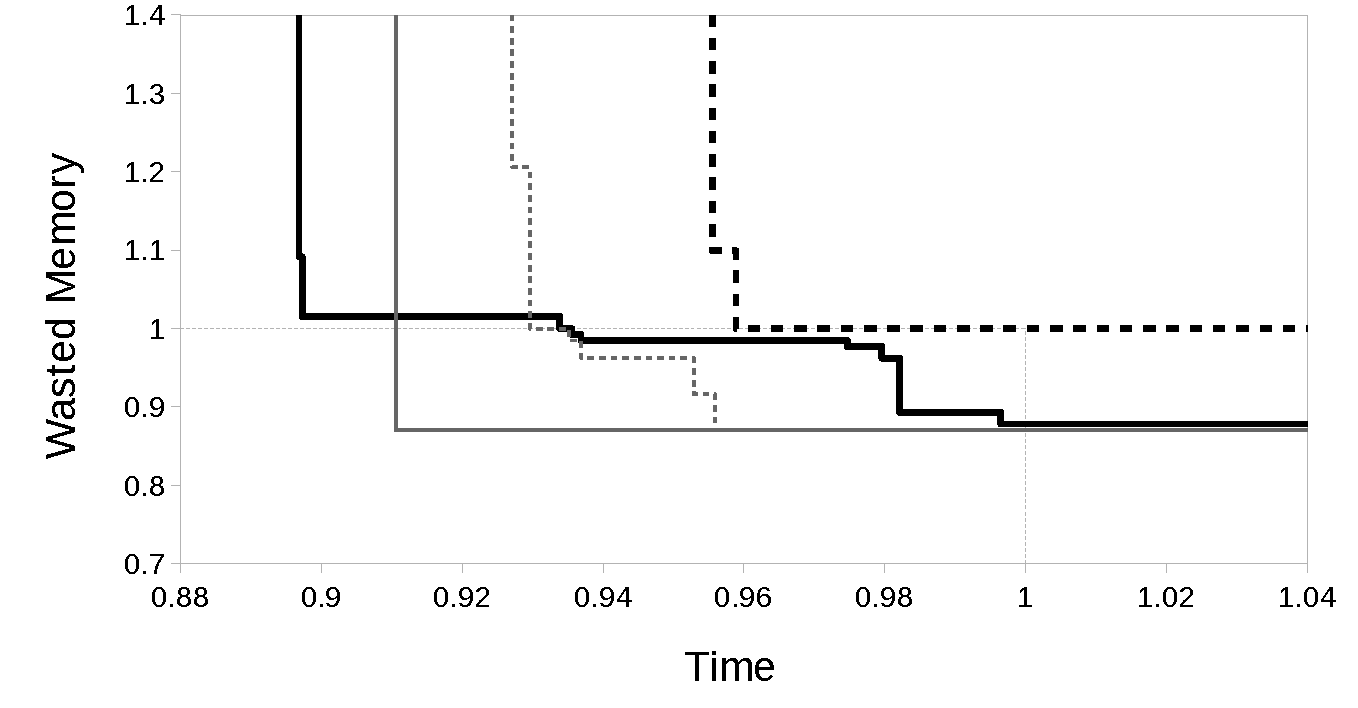
\includegraphics[width=0.47\textwidth]{flex_attainment_pdf}}
	}
	\subfigure[sed]{
		\label{fig_attainment_sed}
		\scalebox{1}{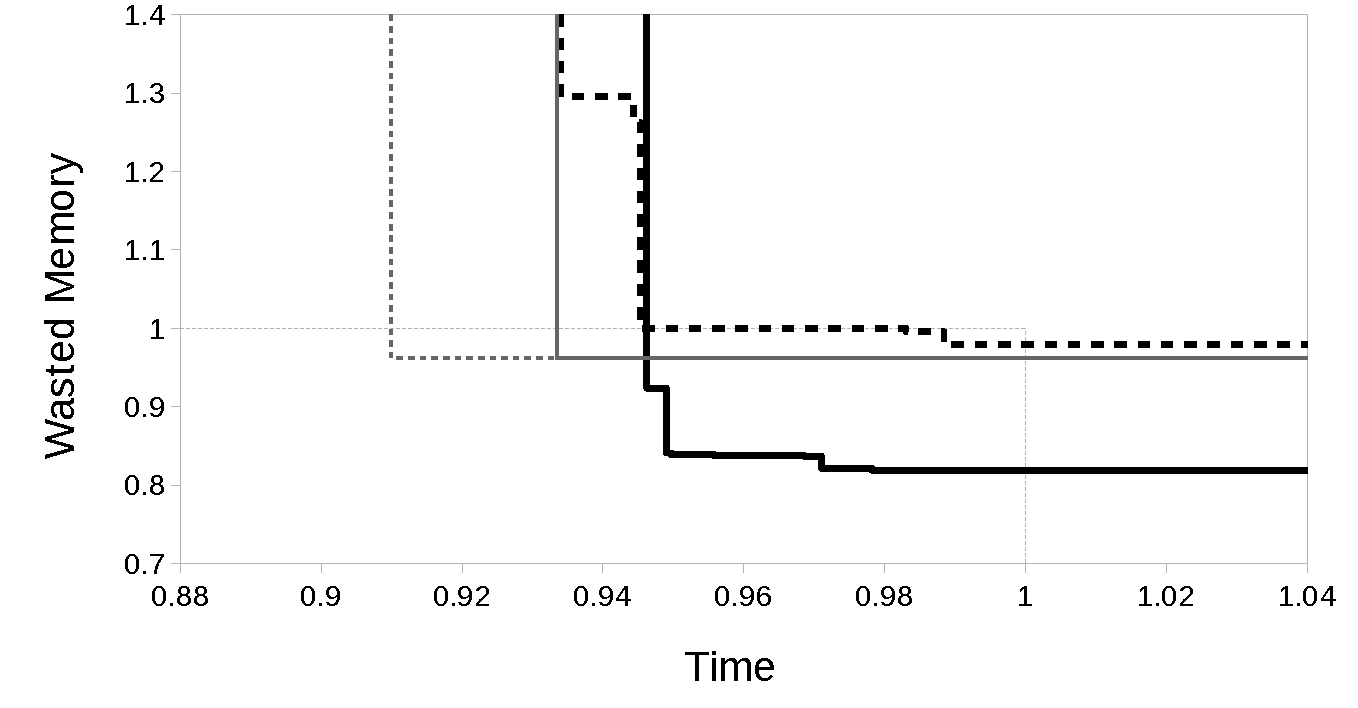
\includegraphics[width=0.47\textwidth]{sed_attainment_pdf}}
	}
	\subfigure{
		\label{fig_attainment_legend}
		
\includegraphics[width=0.45\textwidth]{attainment_legend_pdf}
	}
	\vspace{-1.5em}
	\caption{Combined best solutions from the results of \sr{}, \sn{}, \dr{}, \dn{} over 20 runs for each application. Lower and lefthand solutions dominate high and righthand solutions. `Wasted' memory is memory that is used but not needed.}\label{fig_attainment}
\end{figure*}

To answer RQ1 and RQ2, we first report the 0\%-attainment surfaces (the `reference front' that combines best solutions over all runs) of the results of \sr{}, \sn{}, \dr{} and \dn{} on all subjects in Figure~\ref{fig_attainment}. The solutions are plotted according to their execution time and memory usage (at the `high-water-mark') compared to the original performance. Specially, the original always lies at (1, 1) and is pinpointed by light grey dashed lines. The high-water-mark is our primary target since the remaining non-wasted memory is needed and thus cannot be reduced. 
The figure shows that all algorithms can reduce time or memory consumption without reducing the other objective, implying that the default configuration of \emph{dlmalloc} is not optimal for any application considered. This finding motivates the use of SBSE for tuning memory allocators. In three subjects (\emph{espresso}, \emph{gawk} and \emph{sed}), \dn{} outperforms the other three on memory objective. In terms of time, no algorithm is strictly better and each has its own strengths on different subjects. 
%In Figure~\ref{fig_shallow_random}, we can see that Shallow algorithm is better than Random on subject \emph{sed}, while they are incomparable on the other three subjects. In Figure~\ref{fig_deep_shallow}, Deep algorithm is better than Shallow on three out of four subjects: \emph{espresso}, \emph{gawk}, \emph{sed}, while incomparable on subject \emph{flex}. Notice that unlike other three subjects, Deep can not find solutions have better performance on memory consumption on subject \emph{flex}, and both Shallow and Deep algorithm perform as good as Random, it implies that the optimal solution is very easy to find in the search space. So any search algorithm would fail to ourperform Random search on this special case.

We calculated the Hypervolume and Contribution indicator of each algorithm on every subject, and report them in Figure~\ref{fig_hypervolume} and~\ref{fig_contribution} respectively for all 20 runs. 
In Figure~\ref{fig_hypervolume}, all the values are normalised to the hypervolume of the 0\% attainment reference front, and the closer the value to $1$ is, the better the result is. It is clear that \dn{} outperforms the others on subject \emph{espresso} and \emph{sed} while it performs poorly on subject \emph{flex}, and on subject \emph{gawk} the best value reached by \dn{} is better than that of the others.
%In terms of Hypervolume indicator, Deep algorithm performs the best in general, with an exception on subject \emph{flex}. Shallow algorithm is statistically better than Random on subject \emph{sed}, but there is no significant difference between them on the other three subjects. 
In terms of Contribution, the performance of all algorithms is similar to that of Hypervolume. In general \dn{} is no worse than other algorithms on all subjects but \emph{flex}, where \sn{} has the highest Contribution value.
 
\begin{figure}[htbp]
	\centering
	\subfigure[espresso]{
		\label{fig_hypervolume_espresso}
		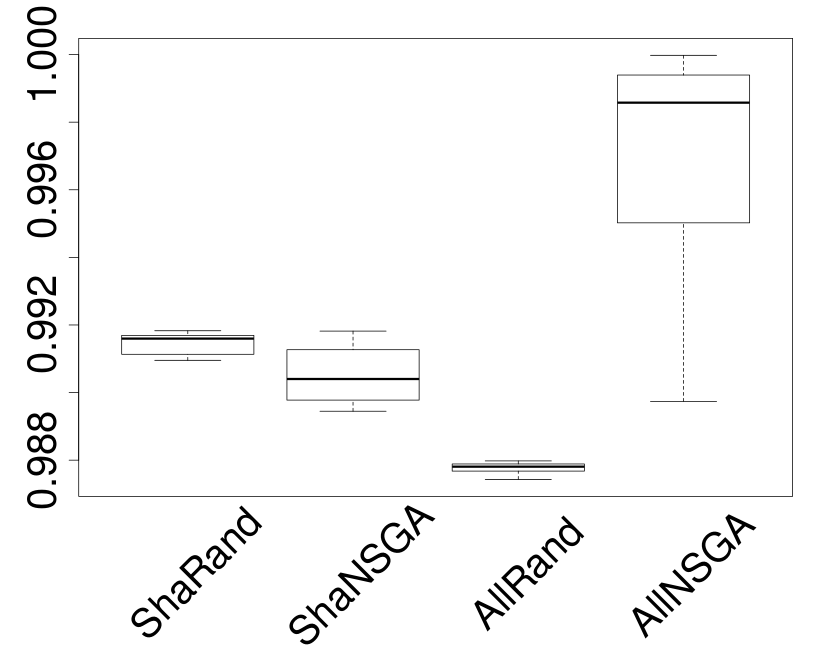
\includegraphics[width=0.22\textwidth]{espresso_hypervolume}
	}
	\subfigure[gawk]{
		\label{fig_hypervolume_gawk}
		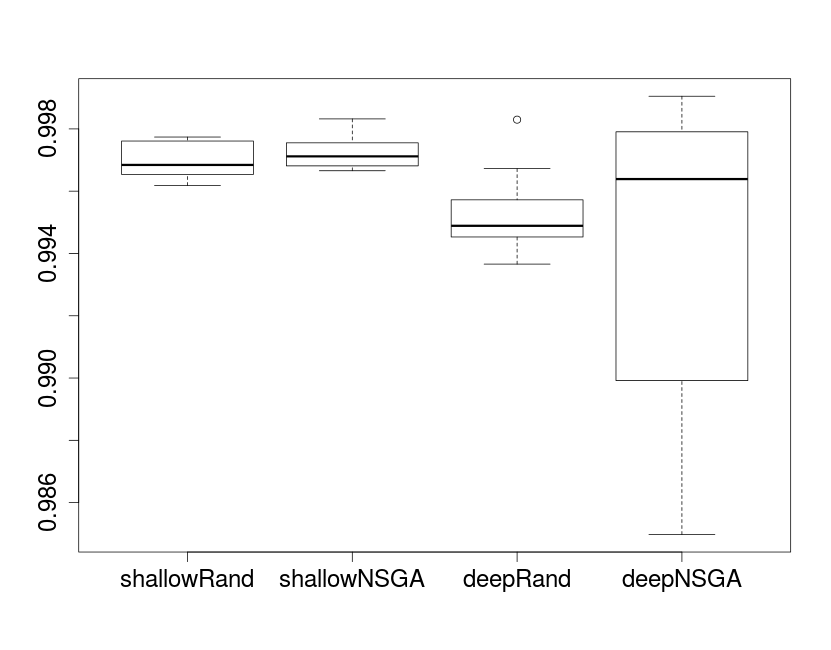
\includegraphics[width=0.22\textwidth]{gawk_hypervolume}
	}
	\subfigure[flex]{
		\label{fig_hypervolume_flex}
		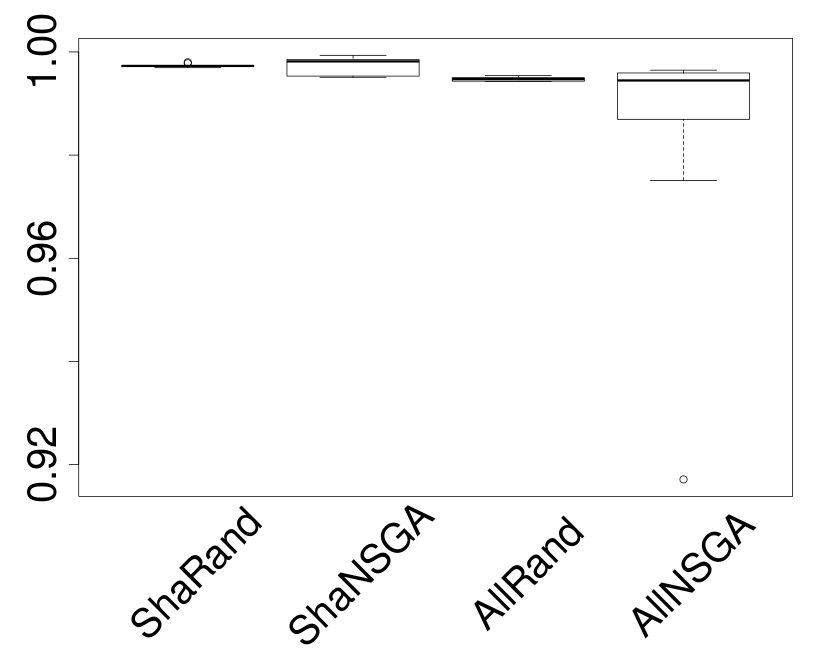
\includegraphics[width=0.22\textwidth]{flex_hypervolume}
	}
	\subfigure[sed]{
		\label{fig_hypervolume_sed}
		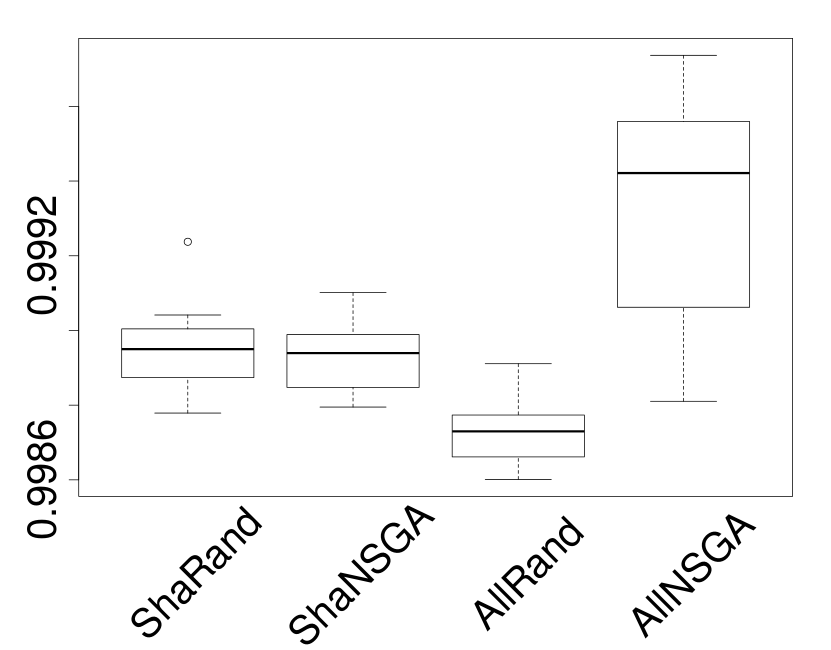
\includegraphics[width=0.22\textwidth]{sed_hypervolume}
	}
	\vspace{-1.2em}
	\caption{Hypervolume indicator of \sr{}, \sn{}, \dr{}, \dn{} on all subjects. Larger values are better.}\label{fig_hypervolume}
\end{figure}

\begin{figure}[htbp]
	\centering
	\subfigure[espresso]{
		\label{fig_contribution_espresso}
		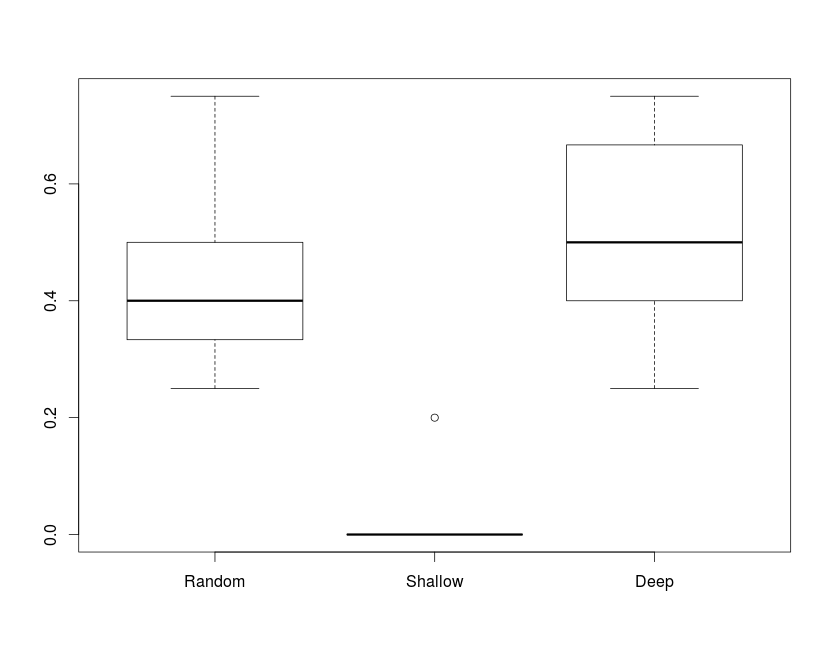
\includegraphics[width=0.22\textwidth]{espresso_contribution}
	}
	\subfigure[gawk]{
		\label{fig_contribution_gawk}
		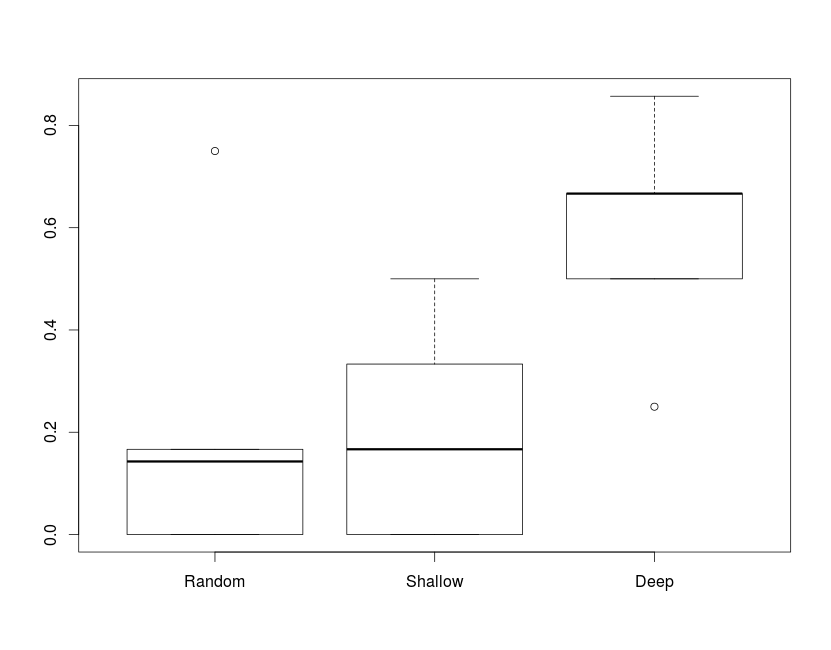
\includegraphics[width=0.22\textwidth]{gawk_contribution}
	}
	\subfigure[flex]{
		\label{fig_contribution_flex}
		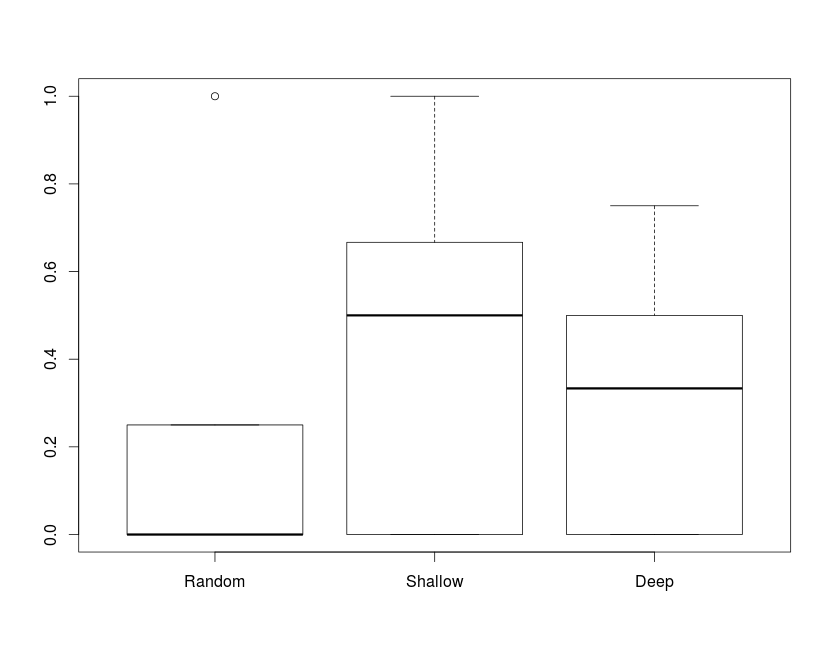
\includegraphics[width=0.22\textwidth]{flex_contribution}
	}
	\subfigure[sed]{
		\label{fig_contribution_sed}
		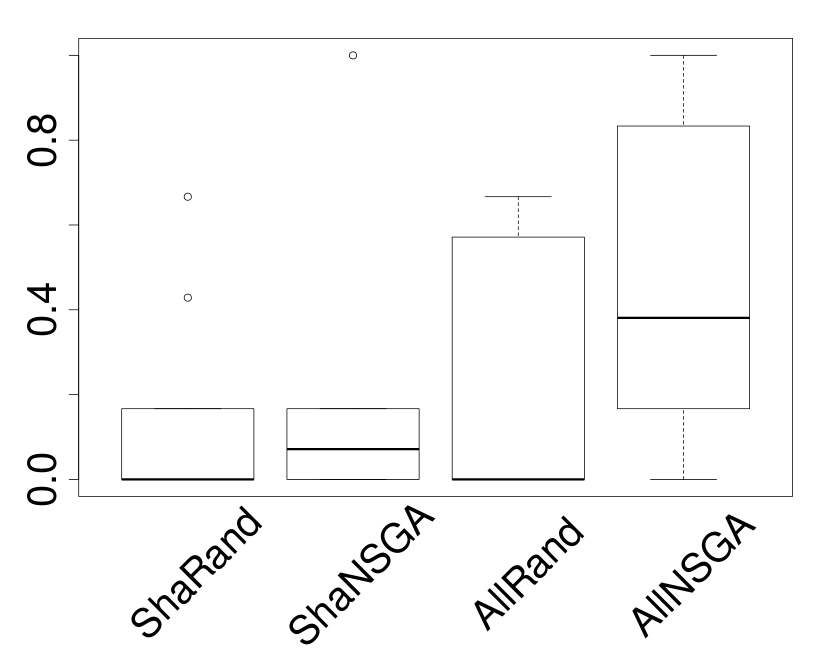
\includegraphics[width=0.22\textwidth]{sed_contribution}
	}
	\vspace{-1.2em}
	\caption{Contribution indicator of \sr{}, \sn{}, \dr{}, \dn{} on all subjects. Larger values are better.}\label{fig_contribution}
\end{figure}

Since \dn{} is good at finding better performance on memory consumption, we report the most memory-saving performance found by each algorithm of each of 20 runs in Figure~\ref{fig_best_memory}. On subject \emph{espresso} and \emph{sed}, \dn{} finds more memory reduction than the other approaches. On \emph{gawk}, it does not perform as consistently, but can also find more memory reduction than other approaches in the best case. 
% FIXME: What does ``potential to do so'' mean here? Please clarify this
% analysis.
% Fan was trying to say, for gawk, though on average AllNSGA doesn't perform as good and stable as other approaches,
% but can occationally outperform other approaches.

%Statistics tests are applied to Hypervolume, Contribution and Best-Memory-Reduction over all subjects.
%We choose Wilcoxon \emph{U}-test because we don't make any assumption on the distributions and the experiments are not paired.
%Considering four approaches on four subjects, we apply Bonferroni Correction (16 tests) to draw conservative conclusions.
%For those \emph{p}-values less than $5\%/16=0.3125\%$, we apply
%Vargha-Delaney effect size measure ($\hat{A}_{12}$) and report the effect sizes in Table~\ref{table_p_value}.
%The effect sizes are all large (effect size larger than $0.79$ or less than $0.21$).

Inferential statistical tests were applied to the Hypervolume, Contribution and Best-Memory-Reduction results over all subjects.
We used the Mann-Whitney-Wilcoxon \emph{U}-test since we make no assumptions about results distributions and apply a Bonferroni Correction (catering for 16 total statistical tests) to draw conservative conclusions with no risk of Type 1 error.
For those \emph{p}-values less than $0.05/16=0.003125$, we apply the
Vargha-Delaney ($\hat{A}_{12}$) effect size measure (see Table~\ref{table_p_value}).
The effect sizes are all large (either above $0.79$ or below $0.21$).

In all experiments involving \emph{\all{}*} we generated and evaluated invalid
configurations (i.e., those that that cause the program to crash). However,
this issue is not specific to our deep-parameter approach: 
surprisingly, even by just tuning the programmer-specified shallow parameters 
(\sr{} and \sn{} optimisations) we {\em also} encounter (and discard) some
configurations that crash the program.
%Unlike shallow parameters, deep parameters are exposed from internal
%sub-expressions that were not monitored or protected by the programmers,
%hence they are expected to cause crashes more often. As a result, the valid
%configurations are sparser in the search space. 
This suggests that SBSE memory allocator tuning can be used as a search based testing technique \cite{mh:icst14-keynote}.
Without any guidance, \dr{}
finds valid configurations less often than \sr{}, and thus requires more
optimisation time than \sr{}. Holding the searches to the same budget means
that \dn{}, which must explore a higher search space, will exhibit a higher
variance. 
% This is also the reason why the performance of \dn{} is not alway
% stable on all subjects. 
Despite this more challenging search space, exposing and optimising deep
parameters still allows \dn{} to find better configurations
than \sn{}.

\begin{figure}[htb]
	\centering
	\subfigure[espresso]{
		\label{fig_best_time_espresso}
		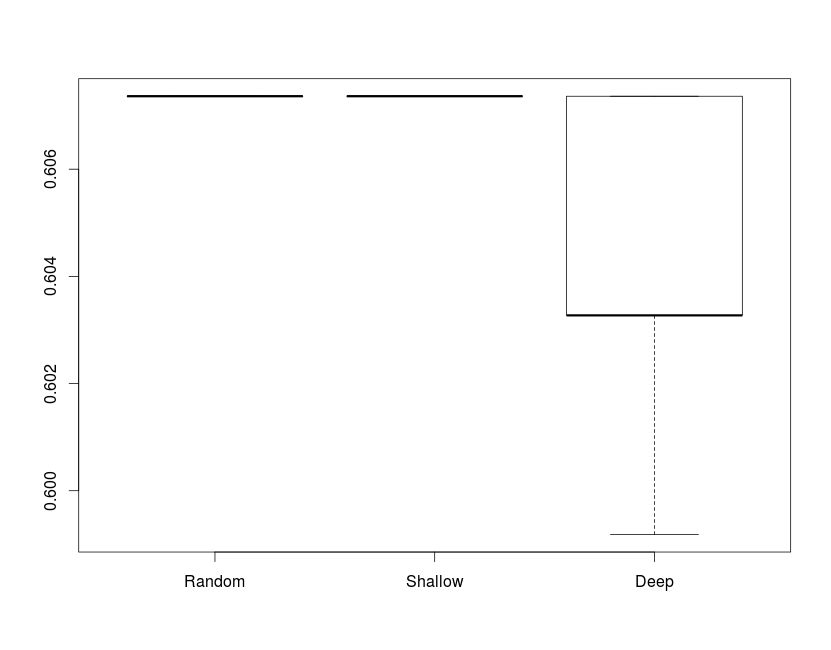
\includegraphics[width=0.22\textwidth]{espresso_best_memory}
	}
	\subfigure[gawk]{
		\label{fig_best_time_gawk}
		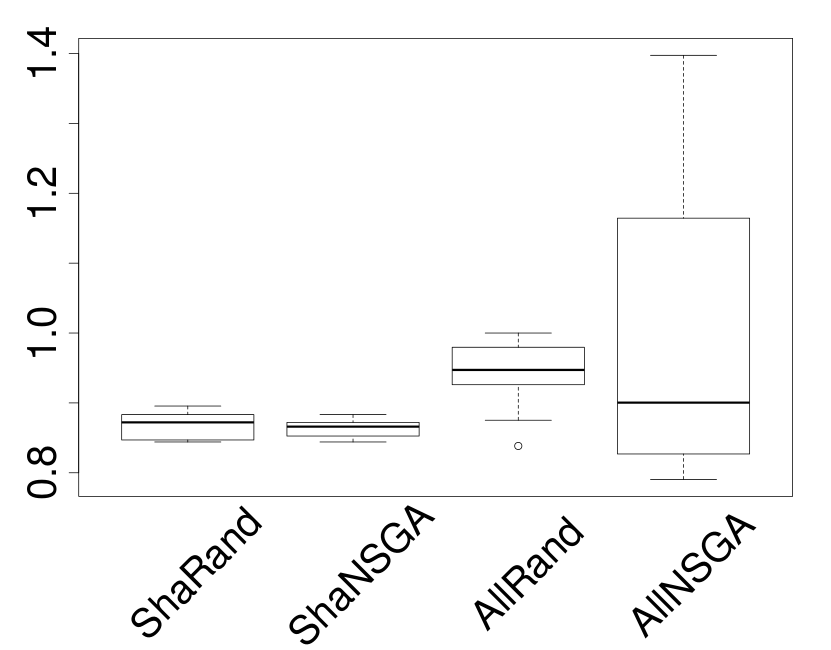
\includegraphics[width=0.22\textwidth]{gawk_best_memory}
	}
	\subfigure[flex]{
		\label{fig_best_time_flex}
		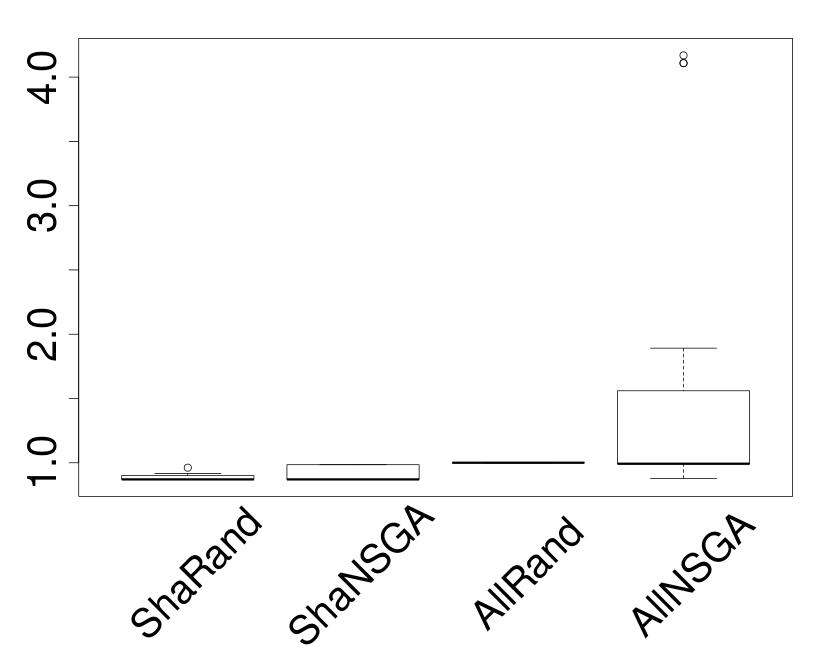
\includegraphics[width=0.22\textwidth]{flex_best_memory}
	}
	\subfigure[sed]{
		\label{fig_best_time_sed}
		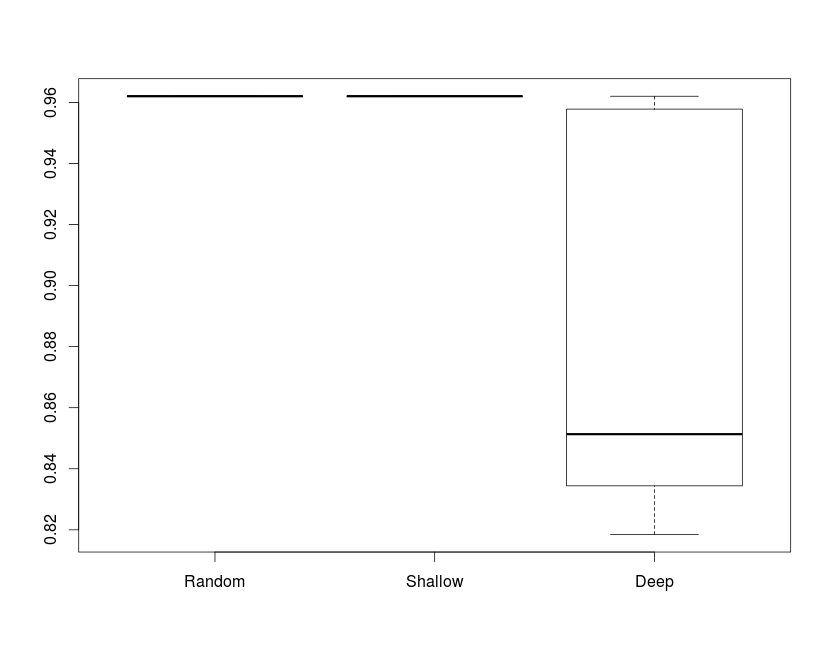
\includegraphics[width=0.22\textwidth]{sed_best_memory}
	}
	\vspace{-1.2em}
	\caption{The least memory consumption found by each algorithm. Smaller numbers are better.}\label{fig_best_memory}
	
	
\end{figure}

\begin{table*}[htb]
\centering
\caption{Vargha-Delaney effect sizes of Hypervolume, Contribution and Best Memory Reduction for any two of the approaches on all subjects. Only the effect sizes of tests with \emph{p}-value less than $5\%/16=0.3125\%$ are reported.}
\label{table_p_value}
\resizebox{0.85\textwidth}{!}{
\begin{tabular}{|l|l|r|r|r|r|r|r|r|r|r|r|r|r|}
\hline
\multicolumn{2}{|l|}{\multirow{2}{*}{Comparing Approachs}} & \multicolumn{4}{c|}{Hypervolume}                                                                             & \multicolumn{4}{c|}{Contribution}                                                                            & \multicolumn{4}{c|}{Best Memory Reduction}                                                                   \\ \cline{3-14} 
\multicolumn{2}{|l|}{}                           & \multicolumn{1}{c|}{\emph{espresso}} & \multicolumn{1}{c|}{\emph{gawk}} & \multicolumn{1}{c|}{\emph{flex}} & \multicolumn{1}{c|}{\emph{sed}} & \multicolumn{1}{c|}{\emph{espresso}} & \multicolumn{1}{c|}{\emph{gawk}} & \multicolumn{1}{c|}{\emph{flex}} & \multicolumn{1}{c|}{\emph{sed}} & \multicolumn{1}{c|}{\emph{espresso}} & \multicolumn{1}{c|}{\emph{gawk}} & \multicolumn{1}{c|}{\emph{flex}} & \multicolumn{1}{c|}{\emph{sed}} \\ \hline
\multirow{3}{*}{\dn{}}              & \dr{}        & 1.000                     & --                        & --                        & 0.975                    & 0.859                     & --                        & --                        & 0.835                    & 0.000                     & --                        & --                        & 0.000                    \\
                                   & \sn{}        & 0.935                     & --                        & 0.105                     & 0.808                    & 0.868                     & --                        & 0.191                     & 0.868                    & 0.063                     & --                        & 0.950                     & 0.050                    \\
                                   & \sr{}        & 0.900                     & --                        & 0.035                     & 0.785                    & 0.814                     & --                        & --                        & 0.875                    & 0.100                     & --                        & 0.979                     & 0.050                    \\ \hline
\multirow{2}{*}{\dr{}}              & \sn{}        & 0.000                     & 0.053                     & 0.038                     & 0.045                    & --                        & --                        & 0.144                     & --                       & 1.000                     & 0.940                     & 1.000                     & 1.000                    \\
                                   & \sr{}        & 0.000                     & 0.070                     & 0.000                     & 0.040                    & --                        & --                        & --                        & --                       & 1.000                     & 0.928                     & 1.000                     & 1.000                    \\ \hline
\multicolumn{1}{|c|}{\sn{}}         & \sr{}        & 0.198                     & --                        & --                        & --                       & --                        & --                        & --                        & --                       & 0.800                     & --                        & --                        & --                       \\ \hline
\end{tabular}
}
\vspace{-1em}
\end{table*}

To enable a more quantitative look at maximal time and memory savings, we
examine the extreme performance observed in our experiments. We report
those that have the best performance on
one objective, even at the cost of reducing performance on the other
objective, found by each
algorithm on each subject and summarise them in Table~\ref{table_best_time_memory}.
Some of these results are significant
departures from the original and are thus not plotted in Figure~\ref{fig_attainment}. 

\begin{table*}[htbp]
\centering
\caption{Best reduction of time or memory (separately) found by each algorithm}
\label{table_best_time_memory}
\resizebox{\textwidth}{!}{
\begin{tabular}{|c|r|r|r|r|r|r|r|r|r|r|}
\hline
\multirow{2}{*}{Subject} & \multicolumn{1}{c|}{\multirow{2}{*}{\begin{tabular}[c]{@{}c@{}}Time\\ Original (s)\end{tabular}}} & \multicolumn{4}{c|}{Time Reduction (\%)} & \multicolumn{1}{c|}{\multirow{2}{*}{\begin{tabular}[c]{@{}c@{}}Memory Original\\ (Peak/Wasted KB)\end{tabular}}} & \multicolumn{4}{c|}{Wasted Memory Reduction (\%)} \\ \cline{3-6} \cline{8-11} 
                         & \multicolumn{1}{c|}{}                                                                               & \sr{}  & \sn{}  & \dr{}  & \dn{} & \multicolumn{1}{c|}{}                                                                                            & \sr{}    & \sn{}    & \dr{}    & \dn{}    \\ \hline
\emph{espresso}                 & 7.24                                                                                                & 1.4      & 1.4      & 1.5     & 1.5     & 3500/521                                                                                                         & 6.1        & 6.1        & 0          & 19.2       \\ %\hline
\emph{gawk}                     & 3.43                                                                                                & 3.2      & 6.7      & 4.4      & 4.4     & 29680/3552                                                                                                       & 15.6       & 15.6       & 16.2       & 20.9       \\ %\hline
\emph{flex}                     & 0.13                                                                                                & 7.9      & 10.0      & 6.2      & 11.6    & 10816/525                                                                                                        & 13.0       & 13.0       & 0          & 12.2        \\ %\hline
\emph{sed}                      & 0.25                                                                                                & 9.4      & 7.0      & 7.0      & 5.4     & 7048/948                                                                                                         & 3.8        & 3.8        & 2.1          & 17.9       \\ \hline
\end{tabular}
}
\vspace{-3mm}
\end{table*}

\begin{table}[htbp]
\centering
\vspace{-1.4em}
\caption{Computation Cost in Time}
\label{table_computation_time}
\resizebox{0.47\textwidth}{!}{
\begin{tabular}{|c|r|r|r|r|r|r|}
\hline
\multirow{2}{*}{Subject} & \multicolumn{4}{c|}{Optimisation Time (h)}                                                                        & \multicolumn{1}{c|}{\multirow{2}{*}{\begin{tabular}[c]{@{}c@{}}Exposing\\ Time (h)\end{tabular}}} & \multicolumn{1}{c|}{\multirow{2}{*}{\begin{tabular}[p{2cm}]{@{}c@{}}Extra Time Needed\\ for \emph{*\nsgaii} (\%)\end{tabular}}} \\ \cline{2-5}
                         & \multicolumn{1}{c|}{\sr{}} & \multicolumn{1}{c|}{\sn{}} & \multicolumn{1}{c|}{\dr{}} & \multicolumn{1}{c|}{\dn{}} & \multicolumn{1}{c|}{}                                                                             & \multicolumn{1}{c|}{}                                                                                                           \\ \hline
\emph{espresso}                 & 39.7      & 46.4     & 9.0      & 39.3     & 12.5                                                                                                    & 18.5                                                                                                                          \\ %\hline
\emph{gawk}                     & 22.7      & 18.4     & 13.9     & 16.4     & 5.4                                                                                                     & 11.7                                                                                                                          \\ %\hline
\emph{flex}                     & 7.7       & 6.3      & 5.3      & 5.0      & 1.3                                                                                                     & 0.7                                                                                                                           \\ %\hline
\emph{sed}                      & 9.4       & 7.6      & 5.9      & 6.6      & 1.9                                                                                                     & 12.6                                                                                                                          \\ \hline
\end{tabular}
}
\end{table}


To answer RQ3, we provide the average optimisation computation time for each of the apporaches in Table~\ref{table_computation_time}. Recall that \dr{} generates and evaluates numerous invalid configurations. However, since crashing or incorrect mutants can be discarded immediately, the computation time of \dr{} is the lowest among all approaches (given a fixed budget in terms of mutants considered). Similarly, \dn{} generates invalid configurations more often than \sn{}, so it costs less computation time than \sn{}. Taking the deep parameter discovery time into account, \dn{} requires slightly more time than \sn{} does, and the percentage of the extra computation time is reported in the last column of Table~\ref{table_computation_time}. Ultimately, \dn{} requires at most 18\% more computation time than \sn{} (on \emph{espresso}), but requires only 0.7\% more computation time on \emph{flex}, on which \dn{} does not perform as good as \sn{}. Overall, since this optimisation step is a compile-time rather than run-time cost and can be done before deployment, we view the benefits of deep parameter optimisation as significantly outweighing their slight additional optimisation time cost.
